\subsection{Функциональная модель программного средства}
\label{sec:domain:model}

Функциональная модель программного средства представлена в виде диаграммы вариантов использования и информационной
модели предметной области. Варианты использования отражают функциональность системы в ответ на внешние воздействия с
точки зрения получения значимого результата для пользователей. Информационная модель предметной области в
дальнейшем будет использоваться при проектировании базы данных для программного средства.

\subsubsection{} Варианты использования программного средства
\label{sec:domain:model:use_cases}

Проектируемое программное средство предполагает, что пользователи делятся на обычных и менеджеров.

Возможности обычного пользователя и менеджера представлены на рисунке \ref{fig:domain:model:use_cases} в виде
диаграммы вариантов использования, разработанной с использованием нотации UML 2.1.

Рассмотрим подробно представленные на рисунке прецеденты.

Регистрация, аутентификация и авторизация – функции, которые доступны для роли «Гость» (пользователь, не
зарегистрированный в системе). В первой версии приложения планируется реализация собственной системы авторизации; в
дальнейшем будет добавлена возможность регистрации с помощью внешних поставщиков данных (Google).

После регистрации пользователь получает доступ к фунциям заполнения профиля. Среди функций заполнения профиля стоит
отметить:

\begin{sidewaysfigure}
  \centering
    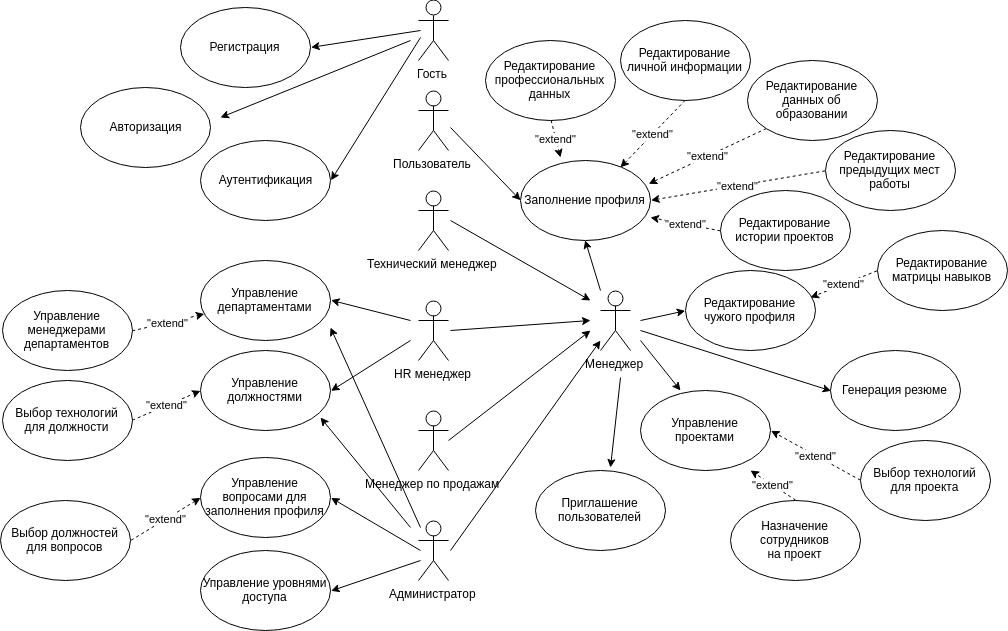
\includegraphics[scale=0.7]{use_case.png} 
    \caption{Диаграмма вариантов использования ПС}
    \label{fig:domain:model:use_cases}
\end{sidewaysfigure}

\begin{itemize}
	\item редактирование личной информации. В эту функцию входит возможность заполнения имени, фамилии, даты рождения,
	адреса электронной почты, места жительства, номера телефона;
  \item редактиование данных об образовании. В этот блок входит возможность ввода учебного заведения или назавния курсов,
  годов начала и конца обучения, возможность указания специализации и ученой степени. Есть возможность добавления
  нескольких мест учебы. Также пользователю предлагается указать свой уровень владения английским языком, что
  является крайне важным фактором при работа в сфере информационных технологий;
	\item редактирование профессиональных данных. В этой секции пользователю предлагается ответить на несколько вопросов,
  связанных с его профессией. Например, разработчику серверной части программного обеспечения будут заданы следующие
  вопросы: "В каких технологиях серверной части ПО вы хороши?", "В каких технологиях клиентской части ПО вы хороши?",
  "С какими базами данных вы имели опыт работы?", "Какие системы управления проектами вы использовали?",
  "С какими методологиями разработки ПО вы знакомы?", "Какие другие инструменты вы использовали в вашей работе?";
	\item редактирование предыдущих мест работы. Здесь можно добавлять предудущие места работы с указанием начала и
  окончания работы. Также есть возможность добавить в свое резюме предудщие рабочие проекты. Здесь можно указать название
  проекта, краткое его описание, зону ответственности, время начала и окончания работы над проектом, роль в команде, 
  а также выбрать из списка технологии, использовавшиеся на данном проекте.
	\item редактирование истории проектов в текущей организации;
\end{itemize}
